\documentclass[12pt,a4paper,oneside]{report}
\usepackage[utf8]{inputenc}
\usepackage[T1]{fontenc}

\usepackage{amsmath}
\usepackage{amsfonts}
\usepackage{amssymb}
\usepackage{graphicx}
\usepackage{fontspec}
\usepackage{titlesec}
\usepackage{tocloft}
\usepackage[margin=2.5cm]{geometry}
\usepackage{lipsum}
\usepackage[skip=10pt]{parskip}
\usepackage{mwe,tikz}
\usepackage{tabto}
\usepackage{dashrule}
\usepackage[backend=biber,style=verbose]{biblatex}
\usepackage{listings,lstautogobble}
\usepackage{scrextend}
\usepackage{enumitem}
\usepackage{hyperref}
\usepackage{float}
\usepackage{wrapfig}
\usepackage{makecell}
\usepackage[german,english]{babel}

\newcommand{\ThRealAuthorNameOne}{Valentin Hörzi}
\newcommand{\ThRealAuthorNameTwo}{Alexander Schörgendorfer}

\newcommand{\ThRealAuthorOneEmail}{valentin.hoerzi@gmail.com}
\newcommand{\ThRealAuthorTwoEmail}{alex.schoergi@gmail.com}

\newcommand{\ThAuthorsClass}{5AHIF}

\newcommand{\ThAuthorOneNumber}{13}
\newcommand{\ThAuthorTwoNumber}{22}


\newcommand{\ThPartner}{Pöttinger Landtechnik GmbH, Industriestraße 1, 4710 Grieskirchen}
\newcommand{\ThPartnerName}{Pöttinger Landtechnik GmbH}
\newcommand{\ThPartnerPersonName}{Dominik Augustin}
\newcommand{\ThPartnerPersonEmail}{Dominik.Augustin@poettinger.at}
\newcommand{\ThSchoolName}{HTBLA Grieskirchen}
\newcommand{\ThPhysicalLocation}{Grieskirchen}
\newcommand{\ThSupervisorName}{Mag. Dipl.-Ing. Rainer Sickinger}
\newcommand{\ThSupervisorEmail}{sickinger@docsced.at}

\addbibresource{citations.bib}

\setcounter{secnumdepth}{3}
\addtolength{\textwidth}{-1cm}
\addtolength{\oddsidemargin}{1cm}
\addtolength{\evensidemargin}{1cm}

\lstset{autogobble=true}
\lstset{language=sh,basicstyle=\ttfamily}
\lstset{language=,basicstyle=\ttfamily}

% C# listing
\definecolor{bluekeywords}{rgb}{0,0,1}
\definecolor{greencomments}{rgb}{0,0.5,0}
\definecolor{redstrings}{rgb}{0.64,0.08,0.08}
\definecolor{xmlcomments}{rgb}{0.5,0.5,0.5}
\definecolor{types}{rgb}{0.17,0.57,0.68}
\lstset{language=[Sharp]C,
	%backgroundcolor=\color{black!10}
	captionpos=b,
	numbers=left, %Nummerierung
	%numberstyle=\tiny, % kleine Zeilennummern
	%frame=lines, % Oberhalb und unterhalb des Listings ist eine Linie
	showspaces=false,
	showtabs=false,
	breaklines=true,
	showstringspaces=false,
	breakatwhitespace=true,
	escapeinside={(*@}{@*)},
	commentstyle=\color{greencomments},
	morekeywords={partial, var, value, get, set},
	keywordstyle=\color{bluekeywords},
	stringstyle=\color{greencomments},
	basicstyle=\ttfamily\small,
}
% end of C# listing

%JavaScript listing (TypeScript)
\lstdefinelanguage{JavaScript}{
	morekeywords=[1]{break, continue, delete, else, for, function, if, in,
		new, return, this, typeof, var, void, while, with},
	% Literals, primitive types, and reference types.
	morekeywords=[2]{false, null, true, boolean, number, undefined,
		Array, Boolean, Date, Math, Number, String, Object},
	% Built-ins.
	morekeywords=[3]{eval, parseInt, parseFloat, escape, unescape},
	sensitive,
	morecomment=[s]{/*}{*/},
	morecomment=[l]//,
	morecomment=[s]{/**}{*/}, % JavaDoc style comments
	morestring=[b]',
	morestring=[b]"
}[keywords, comments, strings]
%end of JS listing

% json listing
\definecolor{delim}{RGB}{20,105,176}
\definecolor{numb}{RGB}{106, 109, 32}
\definecolor{string}{rgb}{0.64,0.08,0.08}

\lstdefinelanguage{json}{
	%backgroundcolor=\color{black!10}
	captionpos=b,
	numbers=left,
	%numberstyle=\small,
	%frame=single,
	%rulecolor=\color{black},
	showspaces=false,
	showtabs=false,
	breaklines=true,
	showstringspaces=false,
	postbreak=\raisebox{0ex}[0ex][0ex]{\ensuremath{\color{gray}\hookrightarrow\space}},
	breakatwhitespace=true,
	basicstyle=\ttfamily\small,
	upquote=true,
	morestring=[b]",
	stringstyle=\color{string},
	literate=
	*{0}{{{\color{numb}0}}}{1}
	{1}{{{\color{numb}1}}}{1}
	{2}{{{\color{numb}2}}}{1}
	{3}{{{\color{numb}3}}}{1}
	{4}{{{\color{numb}4}}}{1}
	{5}{{{\color{numb}5}}}{1}
	{6}{{{\color{numb}6}}}{1}
	{7}{{{\color{numb}7}}}{1}
	{8}{{{\color{numb}8}}}{1}
	{9}{{{\color{numb}9}}}{1}
	{\{}{{{\color{delim}{\{}}}}{1}
	{\}}{{{\color{delim}{\}}}}}{1}
	{[}{{{\color{delim}{[}}}}{1}
	{]}{{{\color{delim}{]}}}}{1},
}
%end of json listing


% Calibri or sans-serif as default font
\defaultfontfeatures{Mapping=tex-text,Scale=MatchLowercase}
\IfFontExistsTF{Calibre}{
	\setmainfont{Calibre}
}{
	\renewcommand{\familydefault}{\sfdefault}
}

% TOC horizontal spacing
\cftsetindents{chapter}{0cm}{1cm}
\cftsetindents{section}{1cm}{1cm}
\cftsetindents{subsection}{2cm}{1.2cm}

% TOC vertical spacing
\renewcommand{\cftchapfont}{
	\bfseries
	\fontsize{13pt}{13pt}
	\selectfont
	\vspace{6pt}
}
\cftbeforechapskip12pt
\renewcommand{\cftsecfont}{
	\fontsize{11pt}{11pt}
	\selectfont
	\vspace{6pt}
}
\cftbeforesecskip6pt
\renewcommand{\cftsubsecfont}{
	\fontsize{10pt}{10pt}
	\selectfont
	\vspace{3pt}
}
\cftbeforesubsecskip6pt

% TOC title
\renewcommand\cfttoctitlefont{
	\hfill
	\fontsize{16pt}{16pt}
	\selectfont
	\bfseries
}
\cftbeforetoctitleskip6pt
\cftaftertoctitleskip12pt

% Title format for chapter, section, sub- and subsubsection
% See https://tex.stackexchange.com/questions/511981/titlesec-vertical-align-chapter-and-section
% The -5pt is just pixel pushing bc I couldn't figure out why my chapter/section/subsection/subsubsection headings are slightly indented
\titleformat{\chapter}[hang]{
	\normalfont
	\bfseries
	\filright
	\fontsize{16pt}{16pt}
	\selectfont
}{
	\makebox[1.7cm][l]{\thechapter}
}{0em}{}
\titlespacing{\chapter}{-5pt}{18pt}{12pt}

\titleformat{\section}[hang]{
	\normalfont
	\bfseries
	\filright
	\fontsize{14pt}{14pt}
	\selectfont
}{
	\makebox[1.7cm][l]{\thesection}
}{0em}{}
\titlespacing{\section}{-5pt}{18pt}{12pt}

\titleformat{\subsection}[hang]{
	\normalfont
	\bfseries
	\filright
	\fontsize{12pt}{12pt}
	\selectfont
}{
	\makebox[1.7cm][l]{\thesubsection}
}{0em}{}
\titlespacing{\subsection}{-5pt}{18pt}{12pt}

\titleformat{\subsubsection}[hang]{
	\normalfont
	\bfseries
	\filright
	\fontsize{11pt}{11pt}
	\selectfont
}{
	\makebox[1.7cm][l]{\thesubsubsection}
}{0em}{}
\titlespacing{\subsubsection}{-5pt}{12pt}{12pt}

% Have list of figures title style be the same as TOC title stile
\renewcommand{\cftloftitlefont}{\cfttoctitlefont}



\newcommand{\SignatureLine}[1]{
	\vskip15pt
	\tabto{9cm}#1
	\vskip10pt
	\tabto{9cm}\hdashrule[0pt][x]{\fill}{.5pt}{.75mm}
}

\newcommand{\BlockCite}[2]{
	\begin{addmargin}[1cm]{0pt}
		#1
		
		\fullcite{#2}
	\end{addmargin}
}

\newcounter{appendix}
\newcommand{\Appendix}[1]{
	\stepcounter{appendix}
	\chapter*{\hspace{\fill}Appendix \Alph{appendix}} \label{app:\Alph{appendix}}
	#1
}

\newcommand{\RefAppendix}[1]{\hyperref[app:#1]{Appendix~#1}}


\title{ERM-Diplomarbeit}
\author{Valentin Hörzi, Alexander Schörgendorfer}

\begin{document}
	
	%%%%%%%%%%%%%%%%%%%%%%%%%%%%%%%%%%%%%%%%%
	%%%   TITELBLATT    %%%%%%%%%%%%%%%%%%%%%
	%%%%%%%%%%%%%%%%%%%%%%%%%%%%%%%%%%%%%%%%%
	\newcommand{\IncludeSchoolTemplate}[2]{
	\vspace*{-7em}
	\makebox[\textwidth]{
		\begin{tikzpicture}[
			every node/.style={anchor=north west,inner sep=0pt},
			x=1mm, y=1mm]
			\node (templatepage) at (0,0)
			{\includegraphics[width=\paperwidth,page=#1]{./summary.pdf}};
			#2
		\end{tikzpicture}
	}
	\newpage
}

\pagenumbering{gobble}

\selectlanguage{german}

\includegraphics[width=\textwidth]{./grafiken/school-header.png}
{\centering
	\vskip1cm
	Fachrichtung Informatik
	\vskip2cm
	Schuljahr 2020/21
	\vskip4cm
	\Huge\textbf{ERM}
	\vskip10pt
	\large
	Gesamtprojekt
	\vskip5pt
	\Huge\textbf{Endkundenportal: Registrierung und Maschinenpark}
	\small
	\vskip4cm
	\begin{flushleft}
		\textbf{Ausgeführt von:}\tabto{9cm}\textbf{Betreuer/Beteuerin:}\linebreak
		\ThRealAuthorNameOne, \ThAuthorsClass-\ThAuthorOneNumber\tabto{9cm}\ThSupervisorName\linebreak
		\ThRealAuthorNameTwo, \ThAuthorsClass-\ThAuthorTwoNumber
		\vskip1cm
		\ThPhysicalLocation, am \today
		\vskip1cm
		\hrule
		Abgabevermerk:\linebreak
		Datum:\tabto{10cm}Betreuer/Beteuerin:
	\end{flushleft}
}



\selectlanguage{german}
\chapter*{\hspace{5pt}Erklärung gemäß Prüfungsordnung}
„Ich erkläre an Eides statt, dass ich die vorliegende Diplomarbeit selbstständig und ohne fremde Hilfe verfasst, andere als die angegebenen Quellen und Hilfsmittel nicht benutzt und alle den benutzten Quellen wörtlich oder sinngemäß entnommenen Stellen als solche kenntlich gemacht habe.“

\ThPhysicalLocation, \today\tabto{9cm}{Verfasser*innen:}
\selectlanguage{english}

\SignatureLine{\ThRealAuthorNameOne}
\SignatureLine{\ThRealAuthorNameTwo}
\newpage
\IncludeSchoolTemplate{1}{
	\node at (77,-28)
		{Informatik};
	\node at (77,-63)
		{\ThRealAuthorNameOne};
	\node at (77,-70)
		{\ThRealAuthorNameTwo};
	\node at (77,-80)
		{2020/21};
	\node at (77,-92)
		{Beispielarbeit};
	\node at (77,-109)
		{\ThPartner};
	\node at (77,-127) [text width=305,align=justify] {
		\fontsize{12pt}{12pt}
		\selectfont
		\par
		Ziel des Projekts war die Entwicklung einer Plattform mit einer i18n und dynamischen Registrierungsmöglichkeit. Kunden können in Zukunft ihre eigenen Maschinen im Endkundenportal hinzufügen. Auch soll es im Endkundenportal verschiedene Benutzergruppen mit dementsprechenden Rechten geben. Das Portal soll verschiedene Funktionen und Berechtigungen darstellen.
		%Im Rahmen der Matura besteht die Aufgabe von ERM darin, eine länderspezifische Registrierung mit jeweiliger Validierung für die Endkunden auf der ganzen Welt bereitzustellen und dieser Prozess soll so einfach und schnell wie möglich für den Benutzer sein. Nach der Registrierung soll jeder registrierte Benutzer einen Maschinenpark anlegen können, wo dieser sich seine eigenen Maschinen speichern kann und somit schnell zu näheren Infos zu diesem Gerät, wie zum Beispiel Highlights, Technische Daten oder Betriebsanleitung, gelangt.
		%\vskip10pt
		\par
		Das Backend soll in C\# und das Frontend in TypeScript realisiert werden.
	};
	\node at (77,-174) [text width=300,align=justify] {
		\fontsize{12pt}{12pt}
		\selectfont
		\par
		Das Registrierungsformular wird im Frontend je nach Länder- und Sprachenwahl dynamisch aufgebaut. Die Auswahl, Anordnung und Validierung variiert je nach Land. Bei erfolgreicher Registrierung über Auth0 wird der User im Backend gespeichert und ihm stehen weitere Features zuverfügung. Die Usereingaben werden im Frontend und im Backend validiert um jegliche Fehler zu vermeiden. Die weiteren Aufrufe sind mit JWT-Tokens gesichert.
		\vskip10pt
		\par
	};
	\node at (77, -222) [text width=300,align=justify] {
		\fontsize{12pt}{12pt}
		\selectfont
		\par
		Das Ergebnis ist ein Endkundenportal, was den User ermöglich, seine Maschinen zu speichern und immer schnell alle wichtigen Informationen darüber herauszufinden. Weiters hat \ThPartnerName \ eine direkte Endkundenverbindung, die es zuvor nicht gab. Dazu wurde das Backend für ein FAQ-Bereich erstellt. Dabei werden die gestellten fragen nach dem beantworten automatisch in 15 Sprachen übersetzt und gespeichert.
	};
}
\IncludeSchoolTemplate{2}{
	\node at (77,-28)
		{Informatik};
	\node at (77,-80){
		
\includegraphics[width=310pt,trim=0pt 0pt 0pt 0pt,clip]{./grafiken/sample_graphic.png}
	};
	\node at (77,-171) [text width=305,align=center]
		{\emph{Screenshot des Programms}};
	\node at (77,-220)
		{--};
	\node at (77,-239)
		{Öffentlich; Bibliothek der \ThSchoolName};
}
\IncludeSchoolTemplate{3}{
	\node at (76,-28)
		{Informatics};
	\node at (77,-63)
		{\ThRealAuthorNameOne};
	\node at (77,-70)
		{\ThRealAuthorNameTwo};
	\node at (77,-80)
		{2019/20};
	\node at (77,-92)
		{Sample Project};
	\node at (77,-109)
		{\ThPartner};
	\node at (77,-125) [text width=305,align=justify] {
		\fontsize{12pt}{12pt}
		\selectfont
		\par
		Ziel des Projekts war die Entwicklung einer Plattform mit einer i18n und dynamischen Registrierungsmöglichkeit. Kunden können in Zukunft ihre eigenen Maschinen im Endkundenportal hinzufügen. Auch soll es im Endkundenportal verschiedene Benutzergruppen mit dementsprechenden Rechten geben. Das Portal soll verschiedene Funktionen und Berechtigungen darstellen.
		%Im Rahmen der Matura besteht die Aufgabe von ERM darin, eine länderspezifische Registrierung mit jeweiliger Validierung für die Endkunden auf der ganzen Welt bereitzustellen und dieser Prozess soll so einfach und schnell wie möglich für den Benutzer sein. Nach der Registrierung soll jeder registrierte Benutzer einen Maschinenpark anlegen können, wo dieser sich seine eigenen Maschinen speichern kann und somit schnell zu näheren Infos zu diesem Gerät, wie zum Beispiel Highlights, Technische Daten oder Betriebsanleitung, gelangt.
		%\vskip10pt
		\par
		Das Backend soll in C\# und das Frontend in TypeScript realisiert werden.
	};
	\node at (77,-173) [text width=300,align=justify] {
		\fontsize{12pt}{12pt}
		\selectfont
		\par
		Das Registrierungsformular wird im Frontend je nach Länder- und Sprachenwahl dynamisch aufgebaut. Die Auswahl, Anordnung und Validierung variiert je nach Land. Bei erfolgreicher Registrierung über Auth0 wird der User im Backend gespeichert und ihm stehen weitere Features zuverfügung. Die Usereingaben werden im Frontend und im Backend validiert um jegliche Fehler zu vermeiden. Die weiteren Aufrufe sind mit JWT-Tokens gesichert.
		\vskip10pt
		\par
	};
	\node at (77, -225) [text width=300,align=justify] {
		\fontsize{12pt}{12pt}
		\selectfont
		\par
		Das Ergebnis ist ein Endkundenportal, was den User ermöglich, seine Maschinen zu speichern und immer schnell alle wichtigen Informationen darüber herauszufinden. Weiters hat \ThPartnerName \ eine direkte Endkundenverbindung, die es zuvor nicht gab.
	};
}
\IncludeSchoolTemplate{4}{
	\node at (76,-28)
		{Informatics};
	\node at (77,-75){
		
\includegraphics[width=310pt,trim=0pt 0pt 0pt 0pt,clip]{./grafiken/sample_graphic.png}
	};
	\node at (77,-166) [text width=305,align=center]
		{\emph{Screenshot of the program}};
	\node at (77,-220)
		{--};
	\node at (77,-240)
		{Public; Library of the \ThSchoolName};
}
	
	\clearpage
	\tableofcontents
	\newpage
	\pagenumbering{arabic}
	
	%%%%%%%%%%%%%%%%%%%%%%%%%%%%%%%%%%%%%%%%%
	%%%   EINLEITUNG    %%%%%%%%%%%%%%%%%%%%%
	%%%%%%%%%%%%%%%%%%%%%%%%%%%%%%%%%%%%%%%%%
	
	\chapter{Einleitung} \label{sec:einleitung}
Aus Gründen der besseren Lesbarkeit wird in dieser Diplomarbeit die Sprachform des generischen Maskulinums angewandt. An dieser Stelle weisen wir darauf hin, dass die ausschließliche Verwendung der männlichen Form geschlechtsunabhängig verstanden werden soll.
\section{Projektteam}
Das Projektteam besteht aus zwei Entwicklern unter denen die Arbeit gleichmäßig verteilt ist.
\subsection{Alexander Schörgendorfer}
Alexander Schörgendorfer, geboren am 04. Oktober 2001 als Sohn von Franz und Renate Schörgendorfer, wohnt in Schlüßlberg in Oberösterreich. Er besuchte von 2008 bis 2012 die Volksschule in Schlüßlberg und von 2012 bis 2016 die damalige Hauptschule 2 in Grieskirchen. Seit September 2016 besucht er die Höhere Technische Bundeslehranstalt in Grieskirchen, Fachrichtung Informatik, und befindet sich derzeit im Maturajahrgang. Alexander Schörgendorfer war besonders für das Backend und den externen Services der Diplomarbeit zuständig.\\
Die Aufgaben von Alexander Schörgendorfer sind eine FAQ Schnittstelle im Backend mit speziellen Berechtigungen, Adressenvalidierung im Backend, Telefonnummernvalidierung im Backend, Login / Logout mit Auth0, sämtliche Pflichtfeldvalidierung im Backend, Suche nach Services, die die benötigten Daten liefern und diese verschiedenen Services vergleichen, Beschaffung der benötigten Daten für den dynamischen Aufbau des Registrierungsformulars von diversen zuvor recherchierten Services. Die gesamte Arbeit soll in DSGVO konformer Form und unter Berücksichtigung des BSI IT-Grundschutzkompendiums vollzogen werden. Das Design des Frontends erfolgt nach der Designvorlage, die von Pöttinger Landtechnik GmbH erstellt worden ist.

\subsection{Valentin Hörzi}
Valentin Hörzi, geboren am 31. Oktober 2001 als Sohn von Christian Strassl und Monika Hörzi, wohnt in Wels in Oberösterreich. Er besuchte von 2008 bis 2011 das Integrative Schulzentrum in Wels bis er schließlich sein letztes Jahr an der Volksschule von 2011 bis 2012 an der Volksschule 3 in der Doktor Schauer-Straße in Wels absolvierte. Von 2012 bis 2016 schloss er die Unterstufe in dem Bundesgymnasium und Bundesrealgymnasium Wels, ebenfalls in der Doktor Schauer-Straße, ab. Seit September 2016 besucht er die Höhere Technische  Bundeslehranstalt in Grieskirchen, Fachrichtung Informatik und befindet sich derzeit im Maturajahrgang. Das Hauptaugenmerk von Valentin galt bei der Entwicklung der Diplomarbeit vor Allem dem Algorithmus, welcher den Aufbau des Registrierungsformulars steuert.
Dieser Algorithmus gewährleistet, dass sich das RF, sowie die Profilübersicht, dynamisch an das jeweilige ausgewählte Land und der derzeitigen Benutzergruppe anpasst. So entsteht die Möglichkeit für amerikanische Benutzer, zusätzlich ihren Bundesstaat auswählen zu können, beziehungsweise italienische Kunden ihre zugehörige Provinz. Dazu wurde auch eine Validierungsmethodik, welche ebenfalls dynamisch auf neue Anforderungen für das RF reagiert, von Valentin entwickelt. Um die Registrierung für den Benutzer so leicht und so schnell wie möglich zu machen, wurden von Valentin auch mehrere Komfortfunktionen eingebaut: automatische Adressvervollständigungsvorschläge, die Beschaffung der Daten des Standorts durch die IP, welche unmittelbar in das RF eingefügt und validiert werden und eine automatische Telefonnummernpräfix-Erkennung.
Auch sorgte Valentin durch eine komplett überarbeitete GitLab Pipeline für eine erhebliche Verbesserung des CI/CD-Geschehens.

\section{Projektbetreuer}

Herr Professor \ThSupervisorName \, war auf Seiten der HTBLA Grieskirchen unsere Ansprechperson. Bei Fragen über das Projekt oder die Diplomarbeit an sich unterstütze er uns.

\section{Auftraggeber}

Die Diplomarbeit wurde in Kooperation mit dem Unternehmen \ThPartnerName \, durchgeführt. Schörgendorfer Alexander kam in den Sommerferien 2019 erstmals durch ein Praktikum mit diesem Unternehmen in Kontakt. Durch diesen Bezug entwickelte sich auch die Zusammenarbeit mit der Diplomarbeit. \ThPartnerName \, wurde 1871 gegründet und produziert Landmaschinen. Der Hauptsitz des Unternehmens liegt in Grieskirchen.

\subsection{Hubert Kerschhuber}

Herr Kerschhuber ist Leiter der Abteilung IT-Softwareentwicklung und war durch diese Position die Hauptansprechperson für die allgemeine Abwicklung der Diplomarbeit.

\subsection{Dominik Augustin}

Herr Augustin war bis Jahresende 2020 unsere Ansprechperson für die technische Abwicklung. Er unterstützte das uns bei jeglichen Fragen über das Projekt und erfüllte jede offene Bitte.

\subsection{Florian Mittlböck}

Herr Mittlböck ist seit Jahresbeginn 2021 unsere Ansprechperson für die technische Abwicklung. Er übernahm ab da an die Stelle von Herrn Augustin in dieser Diplomarbeit.

	
	%%%%%%%%%%%%%%%%%%%%%%%%%%%%%%%%%%%%%%%%%
	%%%   Beispiel    %%%%%%%%%%%%%%%%%%%%%%%
	%%%%%%%%%%%%%%%%%%%%%%%%%%%%%%%%%%%%%%%%%
	
	\chapter{Beispiel} \label{sec:beispiel}

% Example of citing some website
This thesis aims to do the thing\parencite{somewebsite}.

% Example of featuring a graphic
\begin{figure}[h]
	
\includegraphics[width=\textwidth]{./grafiken/sample_graphic.png}
	\vskip0pt
	\caption{Screenshot of the program} \label{fig:samplefigure}
\end{figure}

% Example of featuring codesnippets
\begin{lstlisting}[language=Java]
	public static void main() {
		System.out.println("Hello World");
	}
\end{lstlisting}

See \autoref{fig:samplefigure} and \autoref{sec:introduction}~Introduction.



	
	%%%%%%%%%%%%%%%%%%%%%%%%%%%%%%%%%%%%%%%%%
	%%%   Verwendete Technologien    %%%%%%%%
	%%%%%%%%%%%%%%%%%%%%%%%%%%%%%%%%%%%%%%%%%
	
	\chapter{Verwendete Technologien} \label{technologien}

\section{\LaTeX}
Diese Diplomarbeit wurde mit \LaTeX \space (\textit{{\bf{\textit{La}}}mport {\bf{\textit{\TeX}}}}) verfasst. Dieses Softwarepaket stellt eine Bibliothek von \TeX-Makros dar. \LaTeX \space ist plattformunabhängig und eine gute Möglichkeit gegenüber anderen Textverarbeitungsprogrammen. Dieses Softwarepaket funktioniert nach dem WYSIWYAF-Prinzip (\textit{{\bf{W}}hat {\bf{y}}ou {\bf{s}}ee {\bf{i}}s {\bf{w}}hat {\bf{y}}ou {\bf{a}}sked {\bf{f}}or}), das bedeutet es wird in normalen Textdateien mit Befehlen gearbeitet, die dann in verschiedene Formate (PDF, DVI, PostScript) kompiliert werden können. \autocite{wikiLatex}

\section{BibTeX}
BibTeX erstellt in \LaTeX-Dokumenten Literaturangaben und -Verzeichnisse. Dafür wird eine Literaturdatenbank, ein Textdokument mit der Endung .bib, erstellt, wo jedes Buch, Webseite oder Werk nach einer bestimmten Syntax hineingeschrieben wird. Zur Erstellung eines Verzeichnisses werden aus dem \LaTeX-Dokument alle Zitatverweise herausgesucht und mit der Literaturdatenbank zu einem Werk zugewiesen. Das Verzeichnis wird somit automatisch nach dem eingestellten Stil erstellt. \autocite{wikiBibtex}

\section{TeXstudio}
Die \LaTeX-Dokumente dieser Diplomarbeit wurden mit TeXstudio erstellt. Dieser Editor ist plattformunabhängig und er kompiliert und zeigt Dokumente an. Es besitzt eine Autocomplete-Funktion für \LaTeX-Befehle, Echtzeit-Syntaxkontrolle und -Rechtschreibüberprüfung. Weiteres besteht die Möglichkeit, dass Unicode-kodierte Dateien verarbeitet werden. \autocite{wikiTexstudio}


\section{Twilio} \label{sec:twilio}
Twilio wurde 2008 von Jeff Lawson, Evan Cooke und John Wolthuis in Amerika gegründet. Es betreibt eine Cloud-Kommunikationsplattform als Platform as a Service. Mit den von Twilio zur Verfügung gestellten Dienst, können Entwickler Programmierschnittstellen zum ausführen und empfangen von Anrufen, senden von SMS, verifizieren von Telefonnummern sowie für andere Kommunikationsfunktionen nutzen. In unseren Implementationen half Twilio bei der Verifizierung der von den Benutzer angegebenen Telefonnummern. \cite{twilioWebsite}

\section{Address Validator}
Der Address Validator wurde von Byteplant Software Solutions \& Services entwickelt. Dieses Unternehmen wurde 2003 in Deutschland gegründet. Neben dem Address Validator bieten sie auch einen Email Validator und einen Phone Validator an. Die Adressvalidierung hilft dabei, Informationen über die Zustellbarkeit einer Adresse zu sammeln, Korrekturvorschläge zu präsentieren, falls die Adresse nicht ganz gültig ist und eine einheitliche Adressformatierung nach den nationalen Standards anzubieten. Für eine Überprüfung benötigt man Straße, Stadt, Internationales Länderkürzel und den API-Key. Optional kann man noch mehr, wie beispielsweise Postleitzahl oder die Locale in der man das Ergebnis erhalten möchte, validieren. Als Antwort bekommt man eine Datei im JSON-Format. Aus dieser JSON-Datei ist es möglich, viele Informationen über die Adresse auszulesen. Falls die Adresse gültig ist, bekommt man im Feld Status ein VALID, bei ungültiger Adresse ein INVALID und falls die Überprüfung kein genaues Ergebnis herausgefunden hat, aber eine Adresse gefunden hat, die es sein könnte, ist der Status SUSPECT mit einen Adressvorschlag. Weiteres beinhaltet die Antwort alles von den einzelnen Adressfelder bis hin zu der formatierten Adresse des Landes und den Geografischen Koordinaten. \cite{addressValidator}

\section{Google Translator}
Die Schnittstelle für den Google Cloud Translator wurde von Google LLC entwickelt. Damit kann man schnell Texte in mehr als 100 Sprachen im eigenen Programm übersetzen lassen. Als Antwort der Übersetzung bekommt man den Titel, den Inhalt und die Abkürzung der Sprache. Nun kann man die Übersetzungen speichern und man braucht nur nach der Spachenabkürzung suchen.
\cite{googleTranslator}

\section{Auth0}
Auth0 wurde 2013 gegründet. Der Hauptsitz dieses Unternehmen liegt in Bellevue, Amerika. "Auth0 ist eine Identitätsmanagement Lösung, welche Sie in den Bereichen Authentifizierung, Registrierung und der Speicherung von Userdaten unterstützt. Über Auth0 kann ein Single sign-on von verschiedenen Plattformen und Applikationen (inklusive sozialer Kanäle wie Facebook, LinkedIn und Twitter) realisiert werden. Im Hintergrund können mehrere Datenquellen zum Login verwendet werden (Datenbank, ADFS, LDAP, etc.) Da Auth0 bereits mit einer Vielzahl an Connectors daher kommt, ist der Entwicklungsaufwand um ein Vielfaches kleiner als bei herkömmlichen Projekten." \autocite{auth0}

\section{Visual Studio Code}
Das Frontend dieser Diplomarbeit wurde in Visual Studio Code programmiert. Dieser Quelltexteditor erschien 2015 von Microsoft und arbeitet mit Quelldateien und Ordnern in Workspaces. Es bietet Versionsverwaltung, Autovervollständigung, Debugging und Syntaxhervorhebung. Es unterstützt Programmiersprachen wie Java, C++, C\#, JavaScript, TypeScript, Python und viele mehr. Für Visual Studio Code gibt es Plug-ins, die das programmieren sehr vereinfachen können. \autocite{wikiVisualStudioCode}

\begin{figure}[H]
	\centerline{
		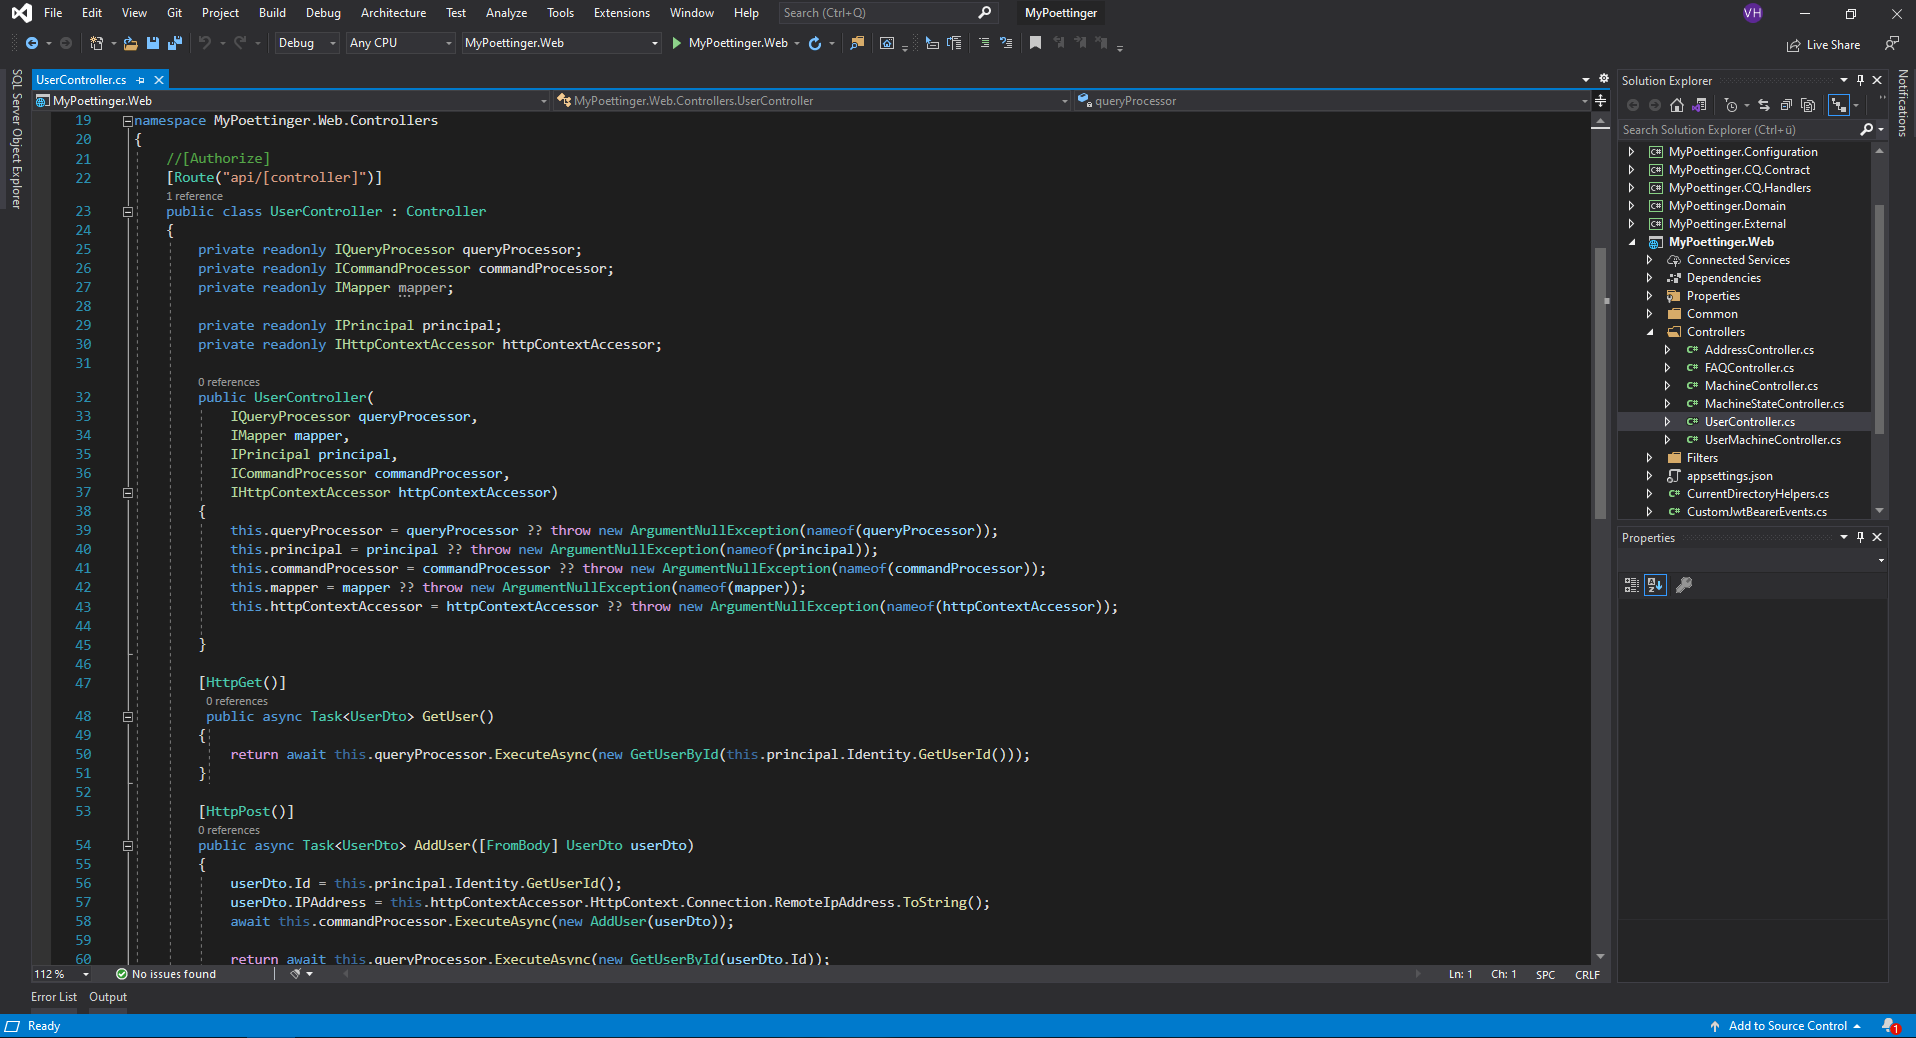
\includegraphics[width=0.8\textwidth]{./grafiken/visual_studio_startview.png}
	}
	\vskip0pt
	\caption{Screenshot vom Startbildschirm von Visual Studio Code} \label{fig:visualStudioCodeStartview}
\end{figure}

\section{Visual Studio 2019}
%Das Backend dieser Diplomarbeit wurde im Visual Studio programmiert. Die von Microsoft stammende Entwicklungsumgebung ist 1997 erschienen und arbeitet mit Projektdateien. Visual Studio bietet viele Funktionen wie IntelliSense, automatische Syntaxprüfung, Debugger mit Bearbeiten und Fortfahren und vieles mehr. Seit 2005 hat es einen integrierten Webserver. Es unterstützt einige Programmiersprachen, wie C\#, C++, C, Visual Basic .NET, TypeScript und viele mehr. \autocite{wikiVisualStudio}

Für das Backend der Diplomarbeit wurde Microsoft Visual Studio gewählt. Diese IDE (Integrated Development Environment) unterstützt den Programmierer durch eine ausgereifte Entwicklungsumgebung mit vielen Features.\\

Am nachfolgenden Screenshot sieht man den Startbildschirm von Microsoft Visual Studio 2019
\begin{figure}[h]
	\centerline{
	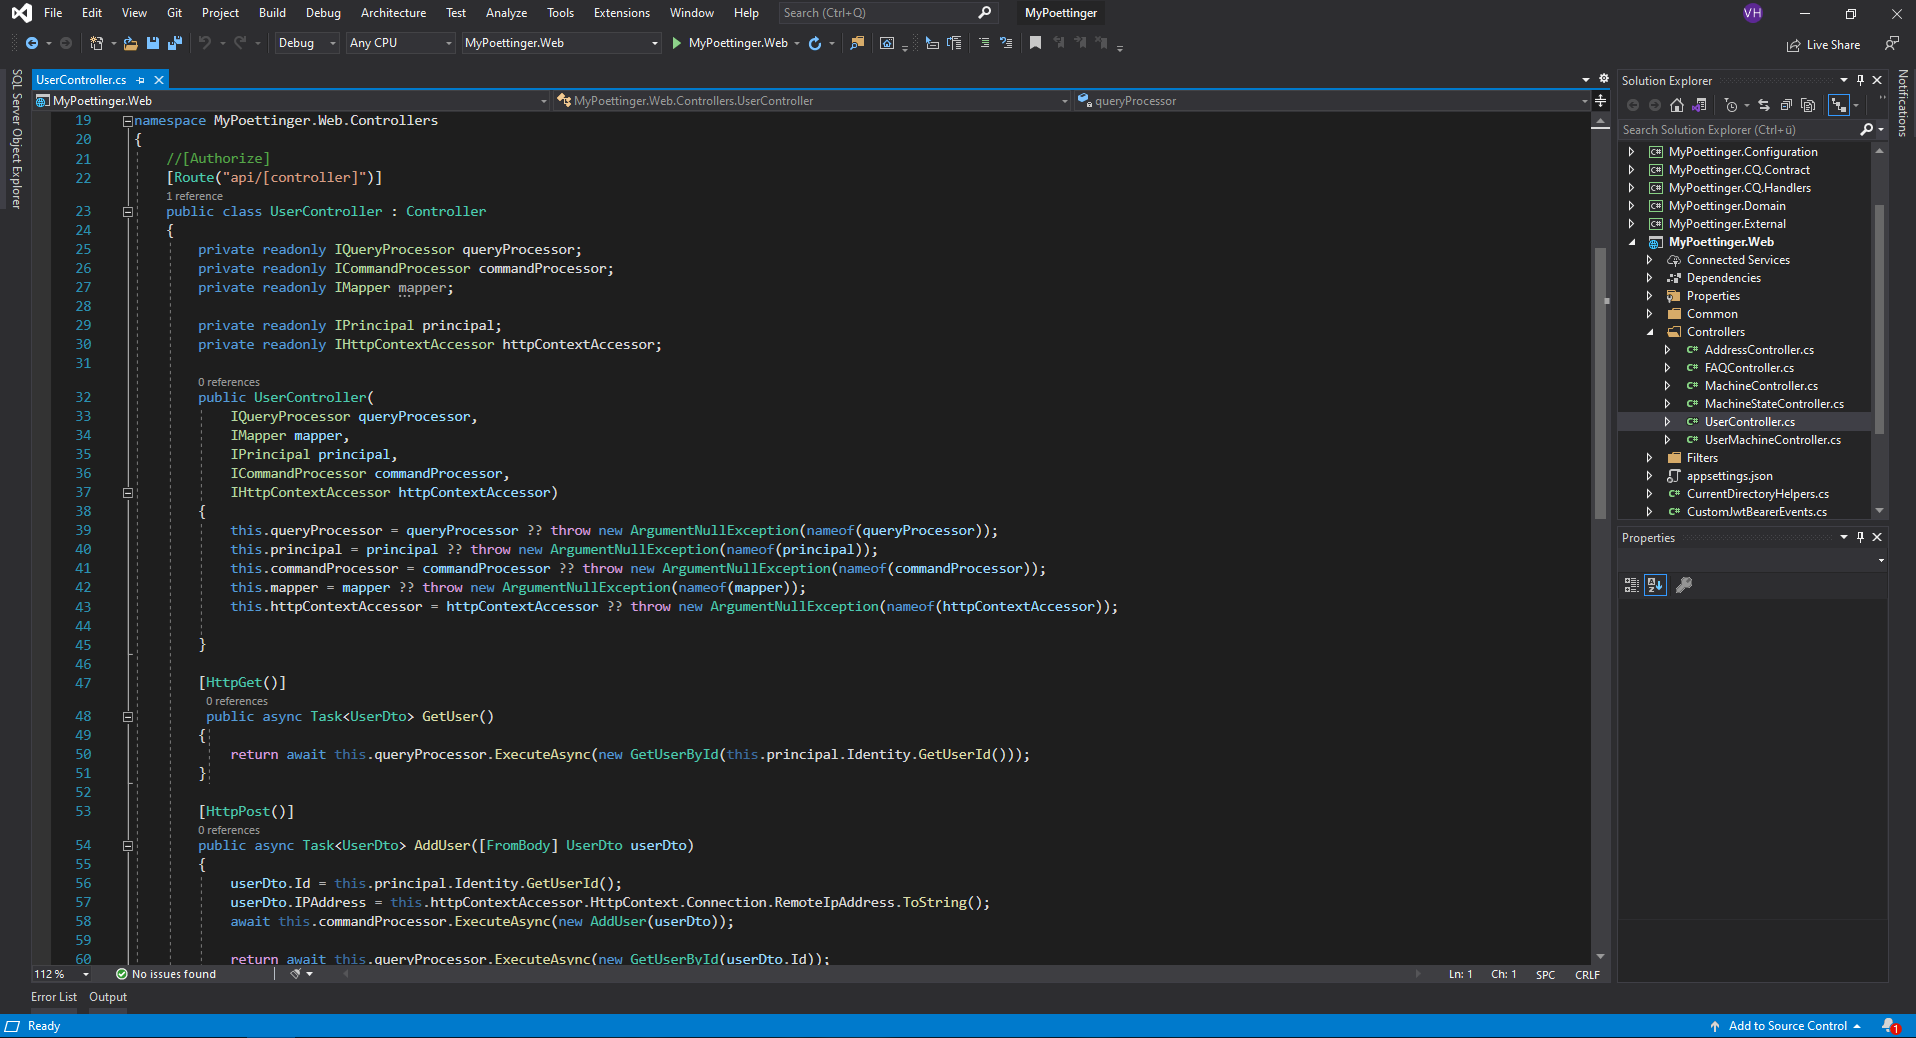
\includegraphics[width=0.8\textwidth]{./grafiken/visual_studio_startview.png}
	}
	\vskip0pt
	\caption{Screenshot vom Startbildschirm von Microsoft Visual Studio 2019} \label{fig:visualStudioStartview}
\end{figure}

Es gibt folgende Editionen von Microsoft Visual Studio 2019, wobei sie sich in den vorhandenen Funktionen unterscheiden:
\begin{itemize}
	\item Community Edition
	\item Professional Edition
	\item Test Professional Edition
	\item Enterprise Edition
\end{itemize}

Diese Diplomarbeit wurde mit der Community Edition erstellt, da diese Version alles zur Verfügung stellt, was gebraucht wurde. \autocite{wikiVisualStudio}

Micrsofot Visual Studio 2019 bietet viele unterstützende Features:
\begin{itemize}
	\item Online-Hilfe, die von der Cursorposition abhängig ist
	\item Ein- und Ausblenden von Codeblöcken
	\item Server-Explorer zum Zugriff auf Datenquellen
	\item Automatische Syntaxprüfung und IntelliSense
	\item Automatische Methoden- und Funktionsergänzung während der Quelltext-Eingabe
	\item Einbindung von Web Services
	\item ActiveX- und .NET-Bibliotheken
    \item Farbliche Kennung von Schlüsselwörtern
    \item Integrierter Debugger mit der Bearbeiten-und-Fortfahren-Funktion
	\item Windows-Nachrichtendienst
	\item WYSIWYG-Editoren zur Benutzeroberflächenentwicklung
\end{itemize}

\section{Postman}
Um die APIs (application programming interface) des Backendes der Diplomarbeit zu testen, wurde Postman verwendet. Postman bietet die Funktion, Http-Requests an jede beliebige URL mit jeder verfügbaren HTTP-Methode zu senden. Somit besteht die Möglichkeit, die programmierten Schnittstellen mit verschiedenen Daten schnell zu testen. Dieses Tool unterstützt SOAP, GraphQL und REST. Des weiteren ist Automated Testing möglich und es lassen sich Endpoints simulieren. Somit kann man das Verhalten der APIs sehr gut beobachten, was es einem Programmierer leichter macht Fehler zu finden. \autocite{postmanDocs} \\
Da das Backend dieser Diplomarbeit mit JWT (JSON Web Token) geschützt ist, ist es bei einem Postman-Request nötig diesen Token in den Header einzufügen, um die API zu testen.  \\
Am nachfolgenden Screenshot sieht man einen Request von Postman.
\begin{figure}[H]
	\centerline{
		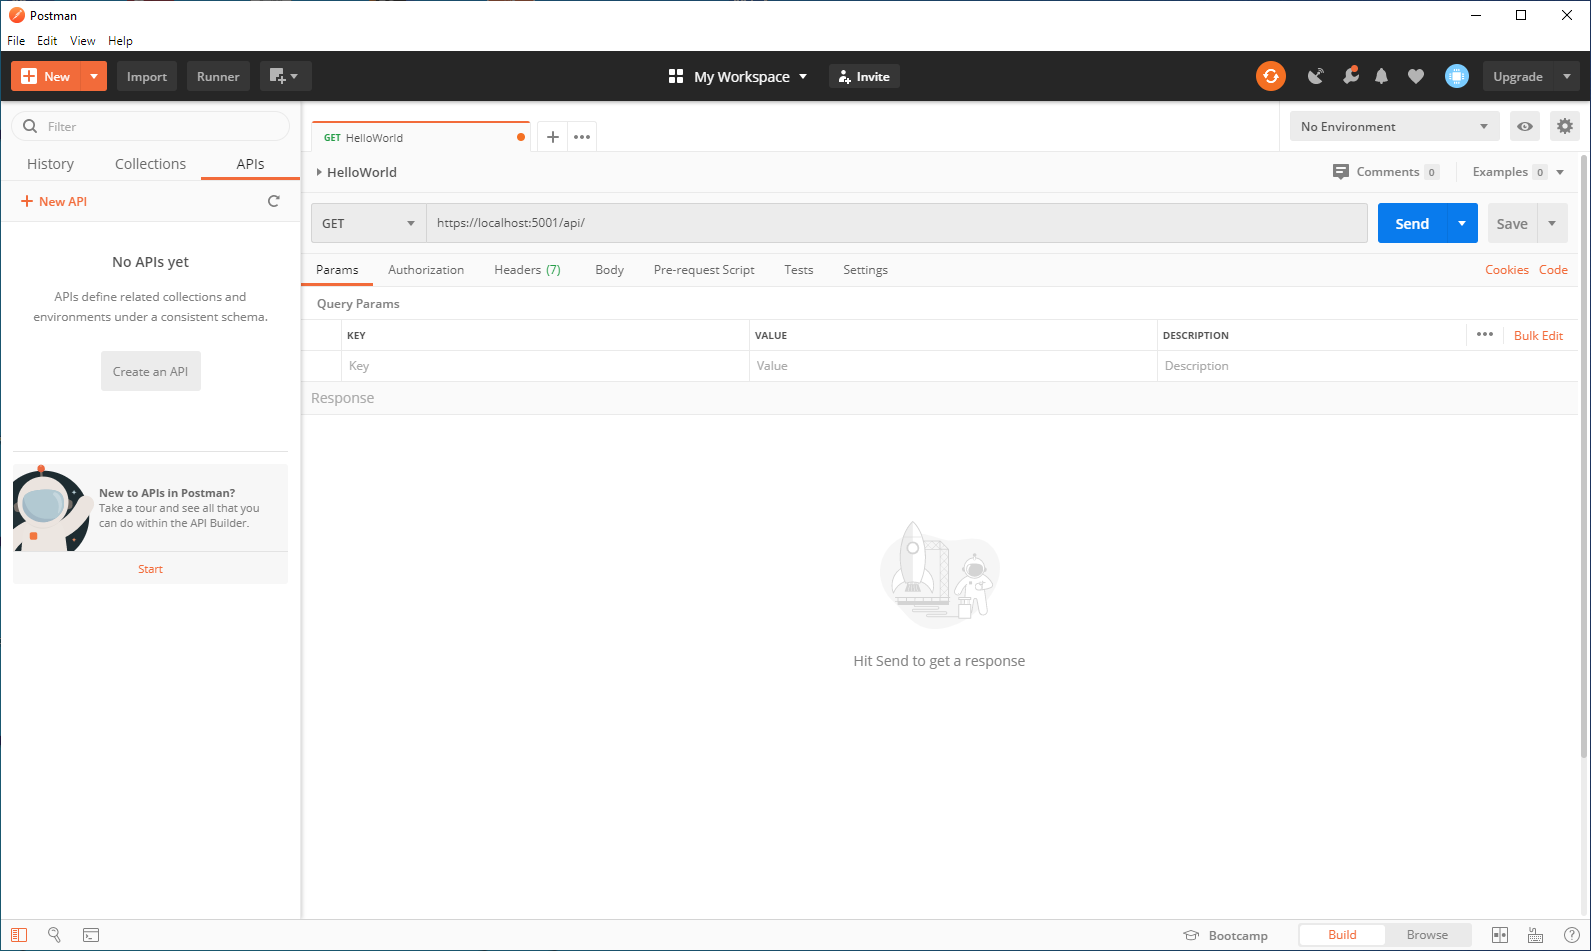
\includegraphics[width=0.8\textwidth]{./grafiken/postman.png}
	}
	\vskip0pt
	\caption{Screenshot von Postman} \label{fig:postman}
\end{figure}

\section{.NET Core 3.1 und C\#}
Für das Backend der Diplomarbeit wurde das Microsoft .NET Framework .NET Core 3.1 verwendet. Die Anwendungen wurden mit der objektorientierten Programmiersprache C\#  erstellt. \autocite{wikiDotnet}

\subsection{.NET Core 3.1}
.NET Core wurde 2015 als Abzweigung vom .NET Framework vorgestellt. Es wurde für eine bessere Modularität und eine leichtere Portierbarkeit auf Microsoft-fremde Plattformen entwickelt. 2016 wurde angekündigt, dass .NET Core mit mehr APIs ausgestatted wird, um die Kompatibilität zwischen verschiedenen .NET Frameworks zu verbessern. \autocite{wikiDotnet} \\
.NET Core 3.1 wurde am 03.12.2019 als Nachfolger von der Version 2.2 veröffentlicht. Dieses Framework unterstützt die Programmiersprachen C#, F#, C++/CLI und Visual Basic .NET. \autocite{wikiDotnetCore}

\subsection{C\#}
C\# wurde von Microsoft entwickelt und 2001 veröffentlicht. Diese plattformunabhängige, objektorientierte Programmiersprache basiert auf Konzepte von den Programmiersprachen Delphi, C, Haskell, C++ und Java.
C\# wird meist nicht gleich von den Compiler in die Maschinensprache, sondern in die Zwischensprache Common Intermediate Language (CIL) übersetzt. \autocite{wikiCSharp}

\begin{lstlisting}[caption={C\#-Syntaxbeispiel},captionpos=b, numbers=left, backgroundcolor=\color{black!10}, language={[Sharp]C}]
using System;
namespace HelloWorld
{
	public class Program
	{
		public static void Main(string[] args)
		{
			Console.WriteLine("Hello World!");
		}
	}
}
\end{lstlisting}

\section{JSON Web Token}
JSON Web Token(JWT) ist ein Access-Token, der auf JSON basiert. Durch JWT kann man verifizierbare Claims austauschen. Mit JWT sind Stateless Sessions möglich, da jede benötigte Information für eine Authentifikation mit dem Token übertragen werden kann. Ein JSON Web Token setzt sich aus dem Header, Payload und der Signatur zusammen. Bei einem Request mit einem Token schreibt man vor dem Token noch "Bearer". \autocite{wikiJWT}

Der Header ist ein JSON-Element. Darin ist gespeichert, welcher Token-Typ es ist und welche Verschlüsselungsmethode angewendet wird. Der Typ ist JWT und als Verschlüsselungsmethoden wird meist HMAC mit SHA-256 oder RSA mit SHA-256 verwendet. \autocite{wikiJWT} \\
\begin{lstlisting}[caption={JWT-Header Beispiel},captionpos=b, numbers=left, backgroundcolor=\color{black!10}, language=json]
{
	"alg": "HS256",
	"typ": "JWT"
}
\end{lstlisting}

Der Payload ist ebenfalls ein JSON-Element. In diesem JSON sind die Claims beschrieben. Es gibt einige reservierte Claims, die den Aussteller, das Subject oder das Ablaufdatum beschreiben, jedoch kann der Aussteller auch einen Private Claim definieren. \autocite{wikiJWT} \\
\begin{lstlisting}[caption={JWT-Payload Beispiel},captionpos=b, numbers=left, backgroundcolor=\color{black!10}, language=json]
	{
		"sub": "8135731594",
		"name": "Max Mustermann",
		"admin": true
	}
\end{lstlisting}

Durch JSON Web Signature(JWS) wird die Signature definiert. Die ist nach RFC 7515 genormt. Mit der im Header festgelegten Hashmethode wir der Header und der Payload Base64 kodierten und durch einem Punkt-getrenntem Format gehasht. Das Ergebnis ist die Signature. \autocite{wikiJWT}

Der JWT-Token setzt sich nun aus dem jeweils Base64-Url kodierten Header, Payload und Signature mit einem Punkt getrennt zusammen. \autocite{wikiJWT} \\
Der Nachfolgende Token setzt sich aus den zwei Beispielen zusammen:\\
\texttt{
eyJhbGciOiJIUzI1NiIsInR5cCI6IkpXVCJ9.eyJzdWIiOiI4MTM1NzMxNTk0IiwibmFtZSI6I\\k1heCBNdXN0ZXJtYW5uIiwiYWRtaW4iOnRydWV9.8NyZnCtWX\_QAlNhfl70zD2tHR\\9j1mtSl9Dwdfnnh60k
}
\section{Angular}
Das Frontend dieser Diplomarbeit wurde mit den Webapplikationsframework Angular geschrieben. Angular ist ein Open-Source-Software, basiert auf TypeScript und wird von einer Online-Community und Google LLC entwickelt.\\
Das Architekturkonzept von Angular ist eine Hierarchie von Komponenten. Durch Module wird Code schneller und Funktionalitäten können ausgelagert werden. TypeScript wird als Entwicklungssprache empfohlen, da diese Generics, statische Typisierung und klassenbasierte objektorientierte Programmierung ermöglicht. \autocite{wikiAngular}
Weiters bietet Angular:

\begin{itemize}
	\item Reaktive Programmierung mit RxJs
	\item Einfaches Routing
	\item Asynchrone Kompilierung von Templates
	\item Dynamisches Laden
	\item Dependency Injection
	\item Lazy- \& Eagerloading
\end{itemize}

\section{TypeScript}
TypeScript wurde von Microsoft entwickelt und 2012 veröffentlicht. Diese Programmiersprache basiert auf den ECMAScript6-Standard. Der TypeScript-Compiler kompliliert den Code in plain-JavaScript, deshalb ist jeder JavaScript-Code auch ein gültiger TypeScript-Code. Somit sind Bibliotheken wie jQuery oder AngularJS auch in TypeScript verwendbar. \autocite{wikiTypeScript} \\

TypeScript bietet viele unterstützende Features:

\begin{itemize}
	\item Klassen
	\item Module
	\item Arrow-Syntax für anonyme Funktionen
	\item Optionale Parameter und Standardparameter
	\item Namensräume
	\item Tupel
	\item Async/Await
	\item Generische Programmierung
	\item Aufzählungstyp
	\item Interfaces
	\item Type Erasure
	\item Typinferenz
	\item Methodensignatur
	\item Enums
\end{itemize}

\begin{lstlisting}[caption={TypeScript-Beispiel Function},captionpos=b, numbers=left, backgroundcolor=\color{black!10},language=JavaScript]
public add(a: number, b: number): number {
	return a + b;
}
\end{lstlisting}

\begin{lstlisting}[caption={TypeScript-Beispiel Klasse},captionpos=b, numbers=left, backgroundcolor=\color{black!10},language=JavaScript]
	class Person {
		private name: string;
		private age: number;
		private salary: number;
		
		constructor(name: string, age: number, salary: number) {
			this.name = name;
			this.age = age;
			this.salary = salary;
		}
		
		toString(): string {
			return `${this.name} (${this.age}): (${this.salary})`;
		}
	}
\end{lstlisting}
\begin{lstlisting}[caption={TypeScript-Beispiel Generische Programmierung},captionpos=b, numbers=left, backgroundcolor=\color{black!10},language=JavaScript]
	function doSomething<T>(arg: T): T {
		return arg;
	}
\end{lstlisting}

\section{Git Versionsverwaltung}
Git wurde 2005 veröffentlicht. Diese Software dient zur verteilten Versionsverwaltung von Dateien. Wichtige Bestandteile von Git sind die Erstellung neuer Entwicklungszweige, den sogenannten Branches und das Zusammenführen von zwei Zweigen. Da es keinen zentralen Server gibt, besitzt jeder Benutzer das gesamte Repository als Kopie lokal. Dadurch benötigt man für fast alle Aktionen keinen Internetzugriff. Mit den Hash-Wert eines Commites wird die History eines Projektes gespeichert. Durch diese Speicherung ist die History gesichert, da es nicht möglich ist, einen Commit zu verändern, der dann den selben Hash-Wert hat. \autocite{wikiGit}

\subsection{GitHub}
Für das Diplomarbeitsdokument wurde GitHub verwendet. GitHub wurde 2008 veröffentlicht und gehört seit 2018 zu Microsoft. Es dient zur Versionsverwaltung von Projekten. Diese Open-Source-Software ermöglicht ein leichtes Branching, Merging und Commiting für alle Entwickler. \autocite{wikiGitHub}

\begin{figure}[h]
	\centerline{
		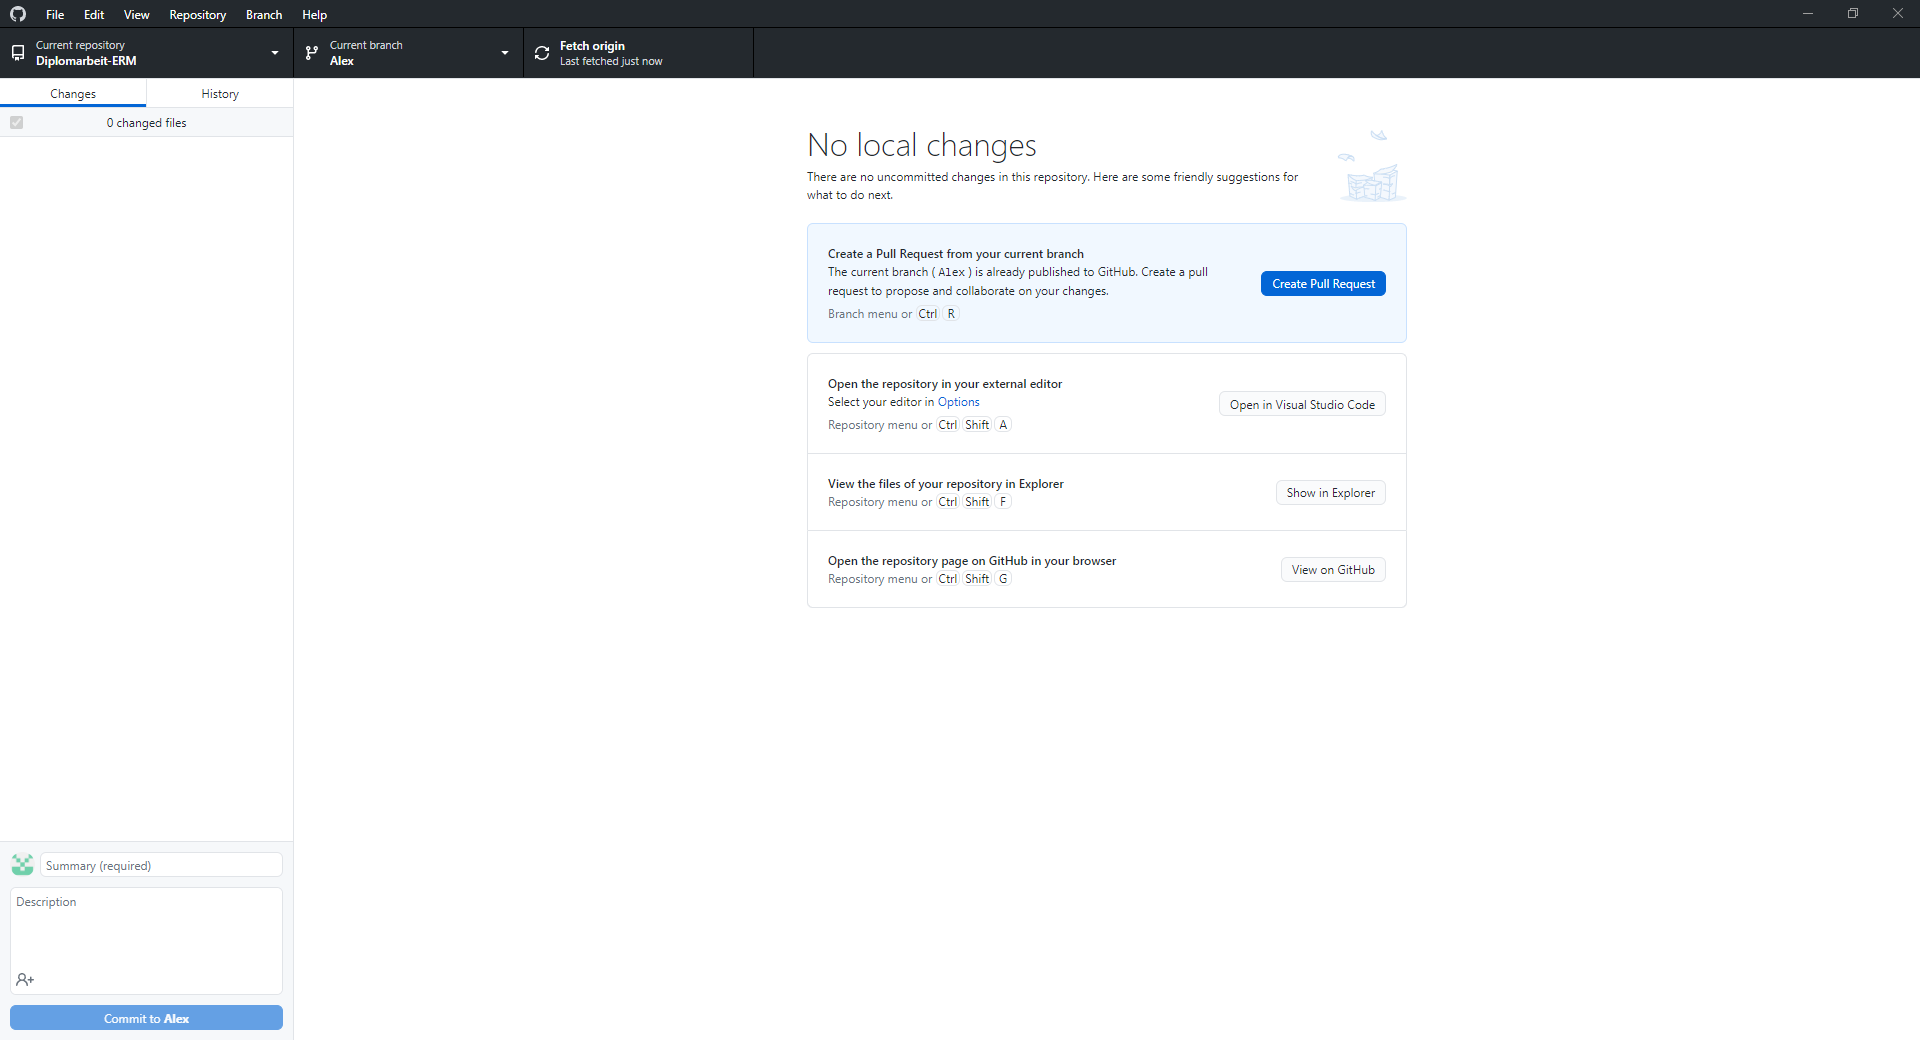
\includegraphics[width=0.8\textwidth]{./grafiken/github_screen.png}
	}
	\vskip0pt
	\caption{Screenshot von GitHub} \label{fig:github}
\end{figure}

\subsection{GitLab}
Für das Projekt der Diplomarbeit wurde GitLab verwendet. Die Versionsverwaltung basiert auf Git und ist eine Webanwendung. Weitere Features von GitLab ist ein Issue-Tracking-System mit einem Kanban-Board, ein Continuous Integration und Continuous Delivery System, eine Projekt-Wiki, eine Container-Registry und eine Multi-Cluster-Verwaltung. GitLab ist eine Open-Source-Software und wird als Software as a Service angeboten. \autocite{wikiGitLab}

\section{zxcvbn}
Um die Passwortstärke herauszufinden, wurde zxcvbn verwendet. Es erkennt und bewertet Passwörter durch Musterabgleich, Vergleich mit häufige Namen und Nachnamen, englische Wörter aus Wikipedia, Fernsehshows und Filme und Wiederholungen und Tastaturmuster. Als Antwort bekommt man Informationen, wie sicher das Passwort ist und ein Feedback mit einer Warnung und einem Tipp, wie man es noch sicherer machen könnte. \autocite{zxcvbn}
	
	%%%%%%%%%%%%%%%%%%%%%%%%%%%%%%%%%%%%%%%%%
	%%%   BIBLIOGRAPHY  %%%%%%%%%%%%%%%%%%%%%
	%%%%%%%%%%%%%%%%%%%%%%%%%%%%%%%%%%%%%%%%%
	
	\printbibliography[title={\hspace{\fill}Bibliography}]
	
	%%%%%%%%%%%%%%%%%%%%%%%%%%%%%%%%%%%%%%%%%
	%%%   BEGLEITPROTOKOLL  %%%%%%%%%%%%%%%%%
	%%%%%%%%%%%%%%%%%%%%%%%%%%%%%%%%%%%%%%%%%
	
	\chapter*{Begleitprotokoll}
\begin{flushleft}
	
	\small
	Thema des übergeordneten komplexen Aufgabenbereichs oder Projekts:
	\linebreak
	\Large
	Beispielarbeit
	\vskip0pt
	\small
	Individuelle Themenstellung:
	\linebreak
	\Large
	Projektdurchführung
	\vskip15pt
	\small
	Betreuer/in:{\large\tabto{4cm}\ThSupervisorName}\linebreak
	E-Mail-Adresse:{\large\tabto{4cm}\ThSupervisorEmail}\linebreak
	Telefonnummer:{\large\tabto{4cm}--}\linebreak
	\vskip15pt
	\small
	Name der Diplomandin/des Diplomanden und Klasse:{\large\tabto{4cm}\ThRealAuthorNameOne, \ThAuthorsClass}\linebreak
	E-Mail-Adresse:{\large\tabto{4cm}\ThRealAuthorNameOne}\linebreak
	Telefonnummer:{\large\tabto{4cm}--}\linebreak
	\vskip15pt
	\small
	Name der Kooperationspartnerin/des Kooperationspartners und Ansprechperson:{\large\tabto{4cm}\ThPartnerName, \ThPartnerPersonName}\linebreak
	E-Mail-Adresse:{\large\tabto{4cm}\ThPartnerPersonEmail}\linebreak
	Telefonnummer:{\large\tabto{4cm}--}\linebreak
	\vskip15pt
	\small
	Teammitglieder:{\large\tabto{4cm}\ThRealAuthorNameOne}
	\vskip15pt
	\fontsize{10pt}{10pt}
	\selectfont
	
	\begin{tabular}{c|c|c|c|c|c}
		\makecell{Datum der\\Besprechung} & \makecell{Teilnehmer/innen\\der Besprechung} & Vereinbarungen & \makecell{Termin zur\\Erledigung} & \makecell{Paraphe\\Betreuer/in} & \makecell{Paraphe\\Schüler/innen} \\ \hline
		26.06.2020 & \makecell{\ThSupervisorName,\\\ThRealAuthorNameOne,\\\ThRealAuthorNameTwo} & \makecell{Implementierung\\Feature 1} & 03.07.2020 & & \\
		03.07.2020 & \makecell{\ThSupervisorName,\\\ThRealAuthorNameOne,\\\ThRealAuthorNameTwo} & \makecell{Feature 2\\CLI, GUI} & 10.07.2020 & & \\
		10.07.2020 & \makecell{\ThSupervisorName,\\\ThRealAuthorNameOne,\\\ThRealAuthorNameTwo} & \makecell{Configuration\\Files, Manual} & 17.07.2020 & & \\
		17.07.2020 & \makecell{\ThSupervisorName,\\\ThRealAuthorNameOne,\\\ThRealAuthorNameTwo} & \makecell{Bug fixes} & 24.07.2020 & & \\
		17.07.2020 & \makecell{\ThSupervisorName,\\\ThRealAuthorNameOne,\\\ThRealAuthorNameTwo} & \makecell{Bug fixes} & 24.07.2020 & & \\
		17.07.2020 & \makecell{\ThSupervisorName,\\\ThRealAuthorNameOne,\\\ThRealAuthorNameTwo} & \makecell{Bug fixes} & 24.07.2020 & & \\
		17.07.2020 & \makecell{\ThSupervisorName,\\\ThRealAuthorNameOne,\\\ThRealAuthorNameTwo} & \makecell{Bug fixes} & 24.07.2020 & & \\
		17.07.2020 & \makecell{\ThSupervisorName,\\\ThRealAuthorNameOne,\\\ThRealAuthorNameTwo} & \makecell{Bug fixes} & 24.07.2020 & & \\
	\end{tabular}
	\vskip35pt
	\fontsize{8pt}{8pt}
	\selectfont
	Datum: \hdashrule[0pt][x]{3cm}{.5pt}{.75mm}
	\hspace{\fill}
	Unterschrift der Schülerin/des Schülers: \hdashrule[0pt][x]{4cm}{.5pt}{.75mm}
\end{flushleft}
\pagebreak
	
	%%%%%%%%%%%%%%%%%%%%%%%%%%%%%%%%%%%%%%%%%
	%%%   LIST OF FIGURES  %%%%%%%%%%%%%%%%%%
	%%%%%%%%%%%%%%%%%%%%%%%%%%%%%%%%%%%%%%%%%
	
	\listoffigures
	\pagebreak
	
	%%%%%%%%%%%%%%%%%%%%%%%%%%%%%%%%%%%%%%%%%
	%%%   LIST OF Listings  %%%%%%%%%%%%%%%%%%
	%%%%%%%%%%%%%%%%%%%%%%%%%%%%%%%%%%%%%%%%%
	\renewcommand{\lstlistlistingname}{Listingverzeichnis}
	\lstlistoflistings	
	\pagebreak
	
	%%%%%%%%%%%%%%%%%%%%%%%%%%%%%%%%%%%%%%%%%
	%%%   APPENDIX  %%%%%%%%%%%%%%%%%%%%%%%%%
	%%%%%%%%%%%%%%%%%%%%%%%%%%%%%%%%%%%%%%%%%
	\Appendix{
		
\includegraphics[angle=90,height=.65\paperheight]{./grafiken/sample_graphic.png}
	}
	
\end{document}
